\chapter{state of the art}

\clearpage


\section{Introduction}
Skin cancer detection has seen significant advancements in recent years, particularly with the integration of deep learning and ensemble methods. This section reviews the state of the art, focusing on recent research that leverages convolutional neural networks (CNNs), mixture of experts, and advanced ensemble strategies for improved diagnostic accuracy.

\section{skin cancer detection}
The Area Under the Receiver Operating Characteristic Curve (AUC) is a widely used performance metric for binary classification tasks. It quantifies the ability of a classifier to distinguish between positive (melanoma) and negative (benign) samples by measuring the area under the ROC curve, which plots true positive rate against false positive rate across all decision thresholds. An AUC of 1.0 indicates perfect discrimination, while an AUC of 0.5 corresponds to random guessing.

This section examines three pivotal contributions to automated melanoma screening, detailing their methodologies, results, and implementation nuances.

\subsection{Knowledge Transfer Protocols (Menegola et al., 2017)}
\textcite{menegola2017knowledge} conducted a systematic evaluation of transfer learning strategies. Their experimental design included:
\begin{itemize}
  \item Pre-training on ImageNet and fine-tuning on the Kaggle Diabetic Retinopathy dataset.
  \item Single-step transfer (ImageNet→Melanoma) vs \\ double transfer (ImageNet→Retinopathy→Melanoma).
  \item Full fine-tuning of all convolutional layers versus training only the final classifier.
\end{itemize}
They reported AUCs of 80.7\% (single transfer) and 84.5\% (double transfer) on the Atlas and ISIC datasets. Table below summarizes their performance metrics.

\begin{table}[h!]
  \centering
  \caption{Transfer learning performance reported by Menegola et al. (2017)}
  \label{tab:menegola-results}
  \begin{tabular}{lccc}
    \hline
    Protocol & Pre-training & Fine-tuning & AUC (\%) \\
    \hline
    Single-step & ImageNet & Classifier only & 80.7 \\
    Double-step & ImageNet + Retinopathy & Full network & 84.5 \\
    \hline
  \end{tabular}
\end{table}

\begin{figure}[H]
  \centering
  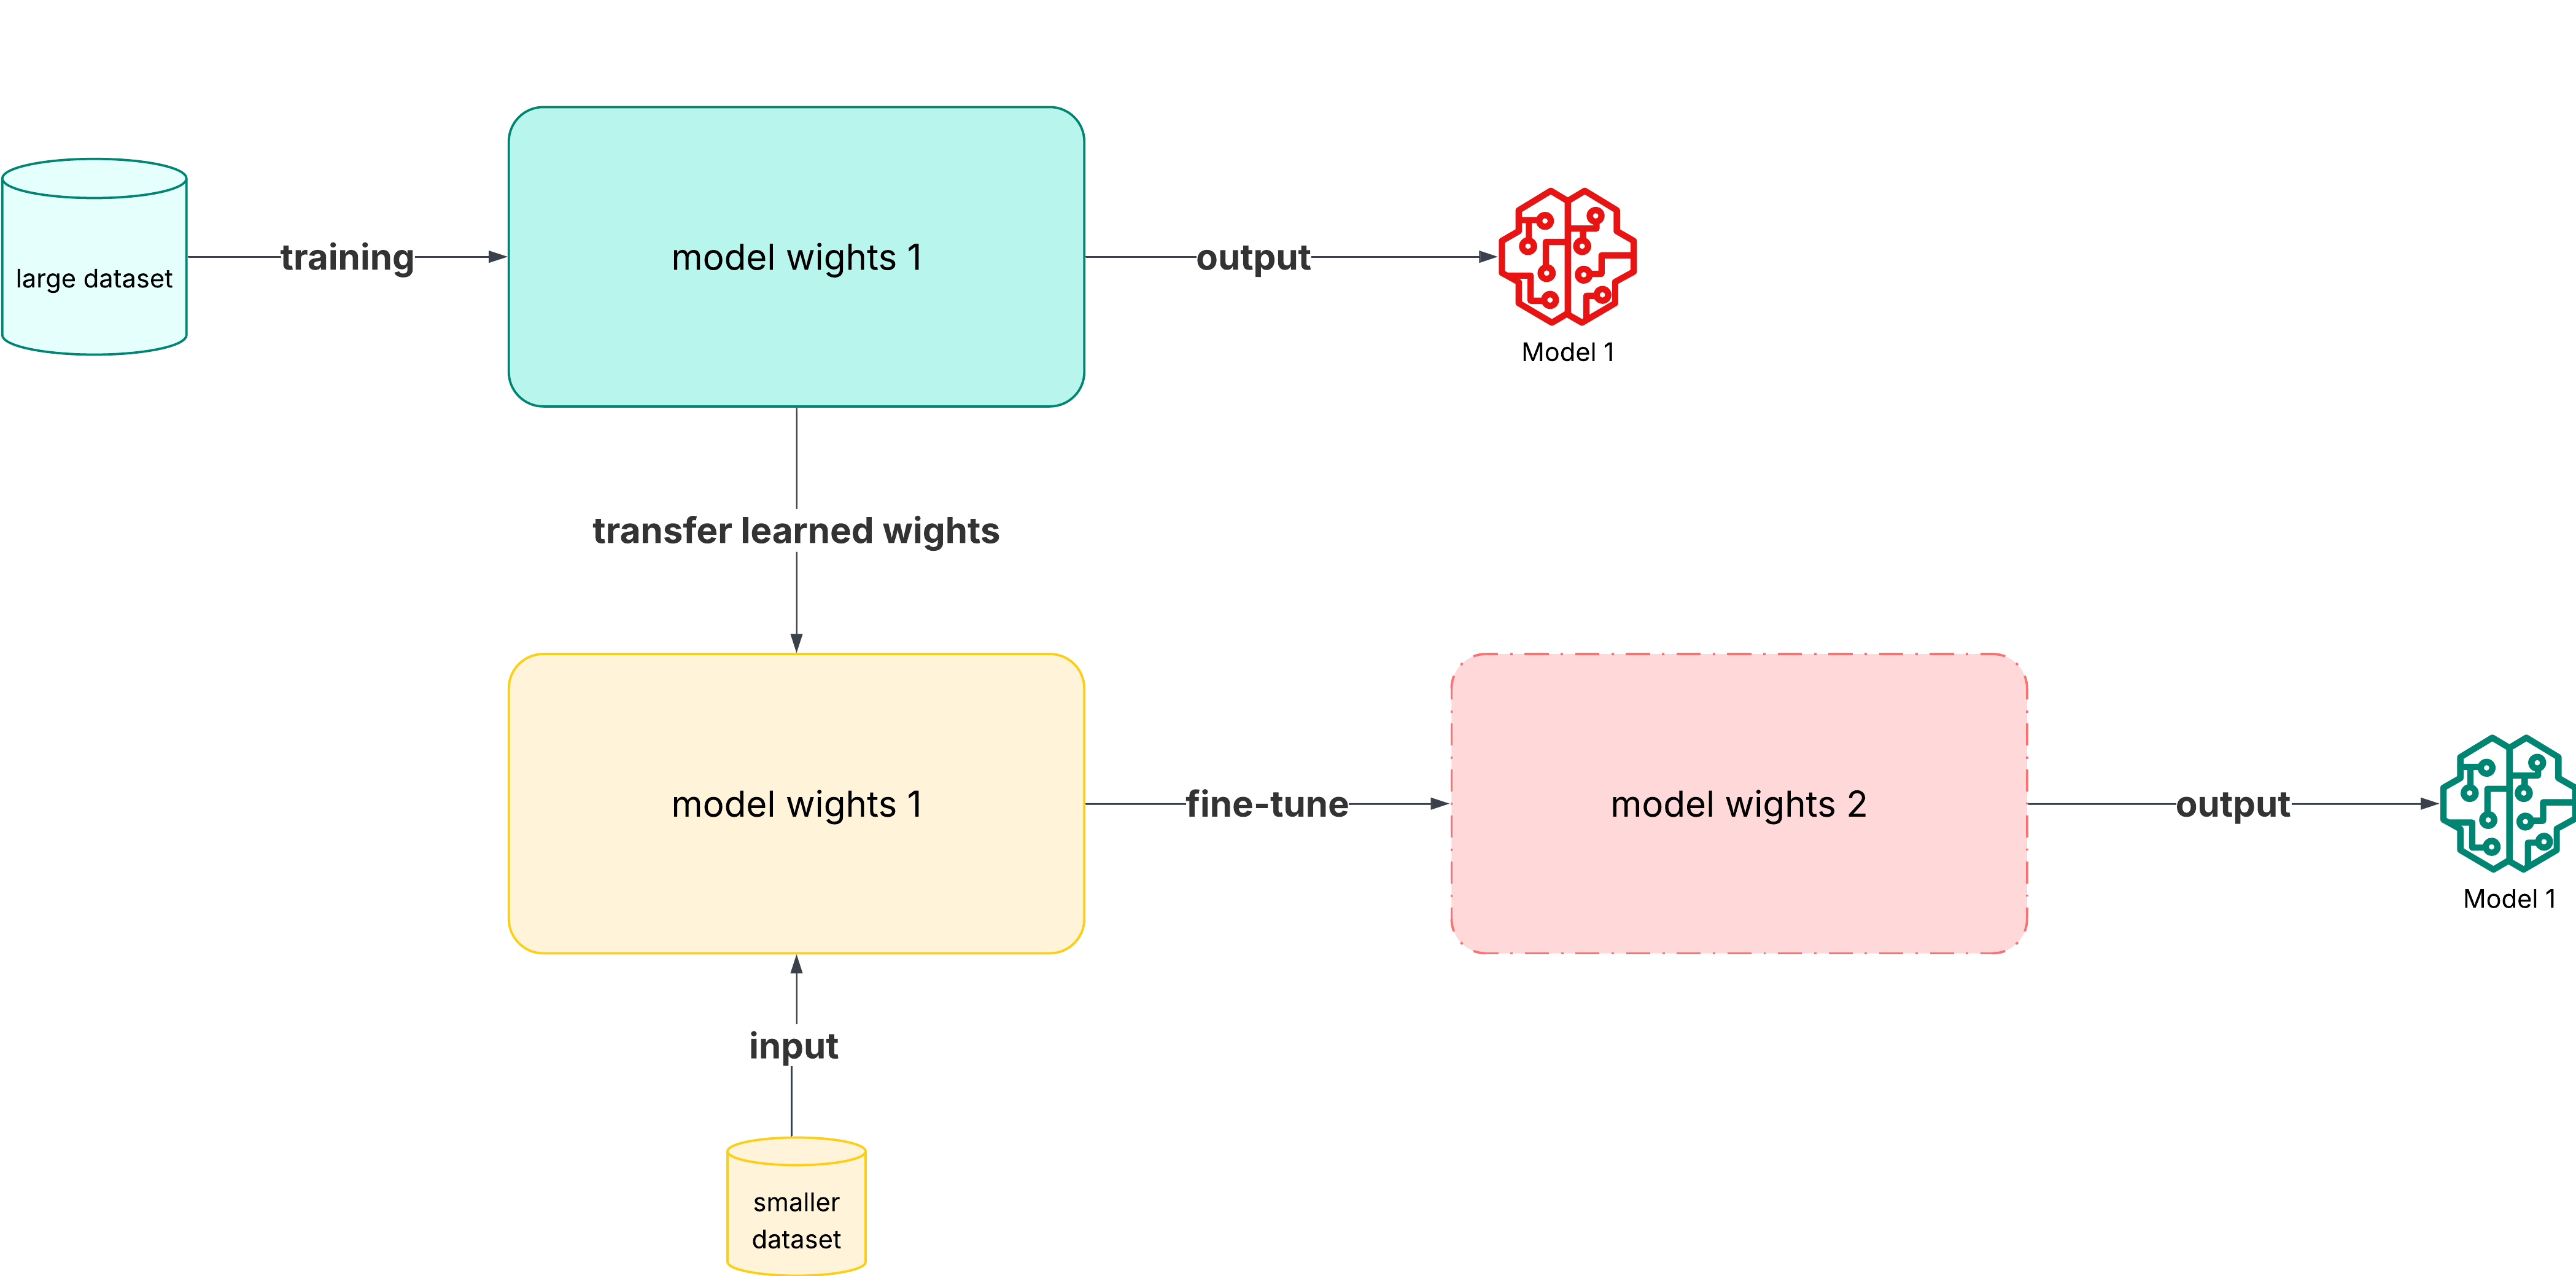
\includegraphics[width=0.7\textwidth]{Transfer_pipeline.png}
  \caption{Schematic exmple of transfer learning pipeline.}
  \label{fig:menegola-pipeline}
\end{figure}

\subsection{EfficientNet Ensemble Approach (Ha et al., 2020)}
\textcite{ha2020efficientnet} proposed an ensemble of diverse EfficientNet backbones, combined with patient-level metadata (age, sex, lesion location). Key aspects include:
\begin{enumerate}
  \item Integration of 9 EfficientNet variants (B0--B8) with varying input sizes.
  \item Use of diagnosis-level labels to refine class definitions.
  \item A two-stage ensemble: model-level averaging followed by meta-classifier stacking.
\end{enumerate}
Their solution achieved a cross-validated AUC of 0.96 on the validation set and 0.94 on the test set, outperforming previous state-of-the-art methods. 


\subsection{Contextual Data Augmentation (DiSanto et al., 2022)}
\textcite{disanto2022contextual} introduced a custom augmentation pipeline targeting real-world variability. Their methodology involved:
\begin{itemize}
  \item Scale jittering to simulate different camera distances.
  \item Random brightness and contrast adjustments for lighting conditions.
  \item Geometric transformations (rotation, perspective warp) to mimic framing differences.
\end{itemize}
They observed a relative increase of 5--7\% in out-of-distribution AUC compared to standard augmentations. Table~\ref{tab:disanto-results} details their comparative study.

\begin{table}[h!]
  \centering
  \caption{Augmentation strategies and performance (DiSanto et al., 2022)}
  \label{tab:disanto-results}
  \begin{tabular}{lcc}
    \hline
    Augmentation set & In-domain AUC & Out-of-domain AUC \\
    \hline
    Standard flips & 0.93 & 0.85 \\
    Contextual pipeline & 0.94 & 0.91 \\
    \hline
  \end{tabular}
\end{table}

\begin{figure}[ht]
  \centering
  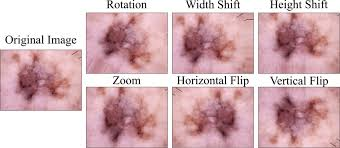
\includegraphics[width=0.5\textwidth]{download.jpg}
  \caption{Examples of image augmentation in skin cancer.}
  \label{fig:disanto-aug}
\end{figure}

\section{mixture of experts}
Mixture of Experts (MoE) is an ensemble strategy that combines multiple specialized sub-models, or "experts," each handling different parts of the input space. A gating network directs each input to one or more experts, allowing the overall model to scale capacity efficiently and focus computation only where needed.

\subsection{Switch Transformer (Fedus et al., 2021)}
\textcite{fedus2021switch} introduced the Switch Transformer, a sparse MoE model for NLP that activates only one expert per token, reducing computational cost while retaining model capacity. Their architecture replaces dense feed-forward layers with MoE layers comprising hundreds of experts and employs a lightweight routing mechanism. To address training instability and communication overhead, they utilize reduced-precision (bfloat16) training and a simplified gating algorithm with dropout safeguarding underutilized experts. The Switch Transformer demonstrates up to 1.8$\times$ speedup in pre-training and strong cross-lingual transfer performance on multilingual benchmarks, scaling to models with over one trillion parameters.

\begin{table}[h!]
  \centering
  \caption{Switch Transformer performance and scaling results (Fedus et al., 2021)}
  \label{tab:switch-transformer}
  \begin{tabular}{lcc}
    \hline
    Model size & Pre-training speedup & Multilingual BLEU \\
    \hline
    200M & 1.2$\times$ & 35.4 \\
    1B & 1.5$\times$ & 37.8 \\
    1T & 1.8$\times$ & 39.2 \\
    \hline
  \end{tabular}
\end{table}

\begin{figure}[H]
  \centering
  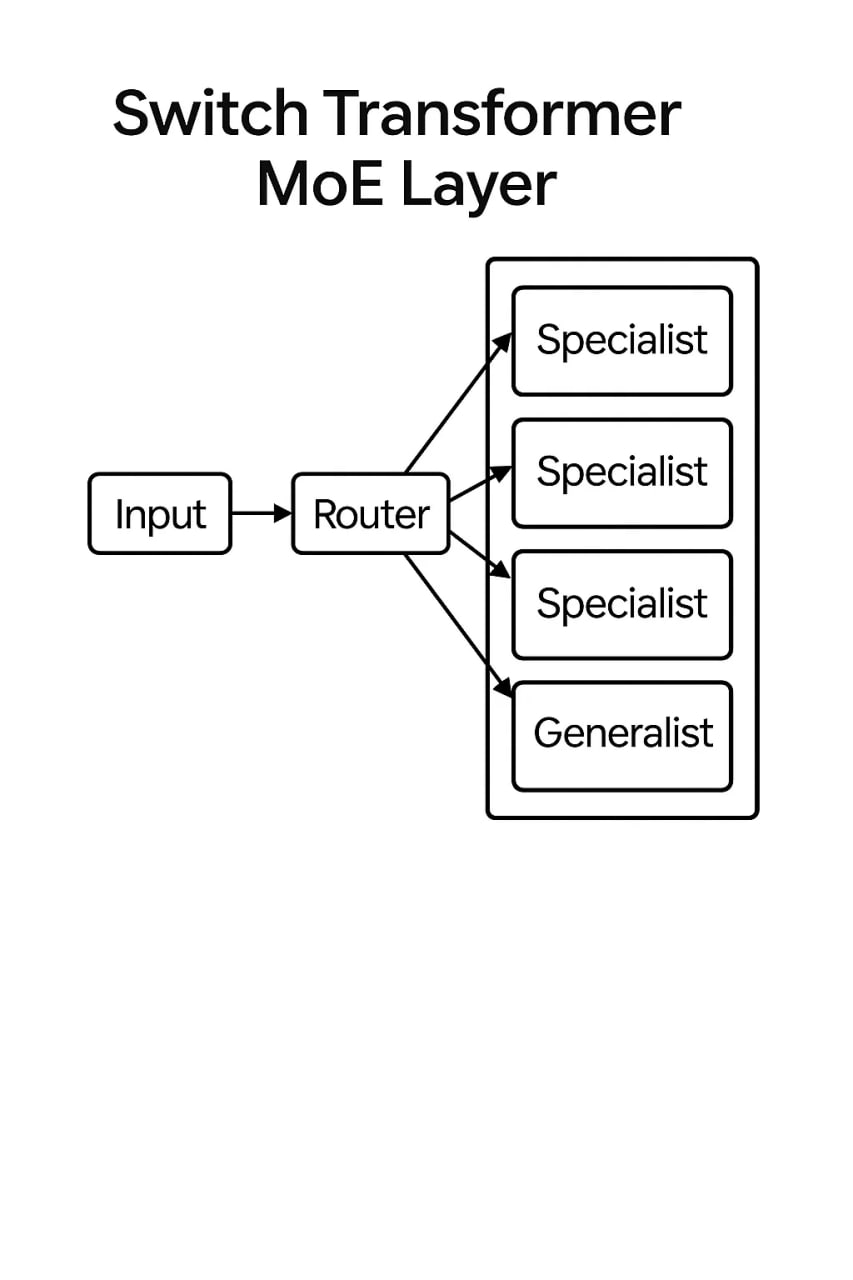
\includegraphics[width=0.5\textwidth]{switch.jpg}
  \caption{diagram of a switch MOE.}
  \label{fig:switch-transformer}
\end{figure}

\subsection{Vision Mixture of Experts (Riquelme et al., 2021)}
\textcite{riquelme2021scaling} extended sparse MoE to computer vision by integrating MoE feed-forward layers into Vision Transformers, creating the V-MoE model. They introduce an adaptive routing strategy that allocates more experts to complex inputs and fewer to simpler ones, enabling dynamic computational budgets. Trained on ImageNet-21k and fine-tuned on ImageNet, V-MoE achieves comparable or better top-1 accuracy than dense ViTs while using 30\% less FLOPs. The largest variant with 15B parameters attains over 90\% top-1 accuracy on ImageNet.

\begin{table}[h!]
  \centering
  \caption{V-MoE accuracy and efficiency comparison (Riquelme et al., 2021)}
  \label{tab:vmoe-results}
  \begin{tabular}{lccc}
    \hline
    Model size & Params & ImageNet top-1 & FLOPs ($\times10^9$) \\
    \hline
    ViT-B/16 & 86M & 0.779 & 55 \\
    V-MoE-B/16 & 86M+Experts & 0.792 & 38 \\
    V-MoE-L/16 & 15B & 0.903 & 85 \\
    \hline
  \end{tabular}
\end{table}

\begin{figure}[ht]
  \centering
  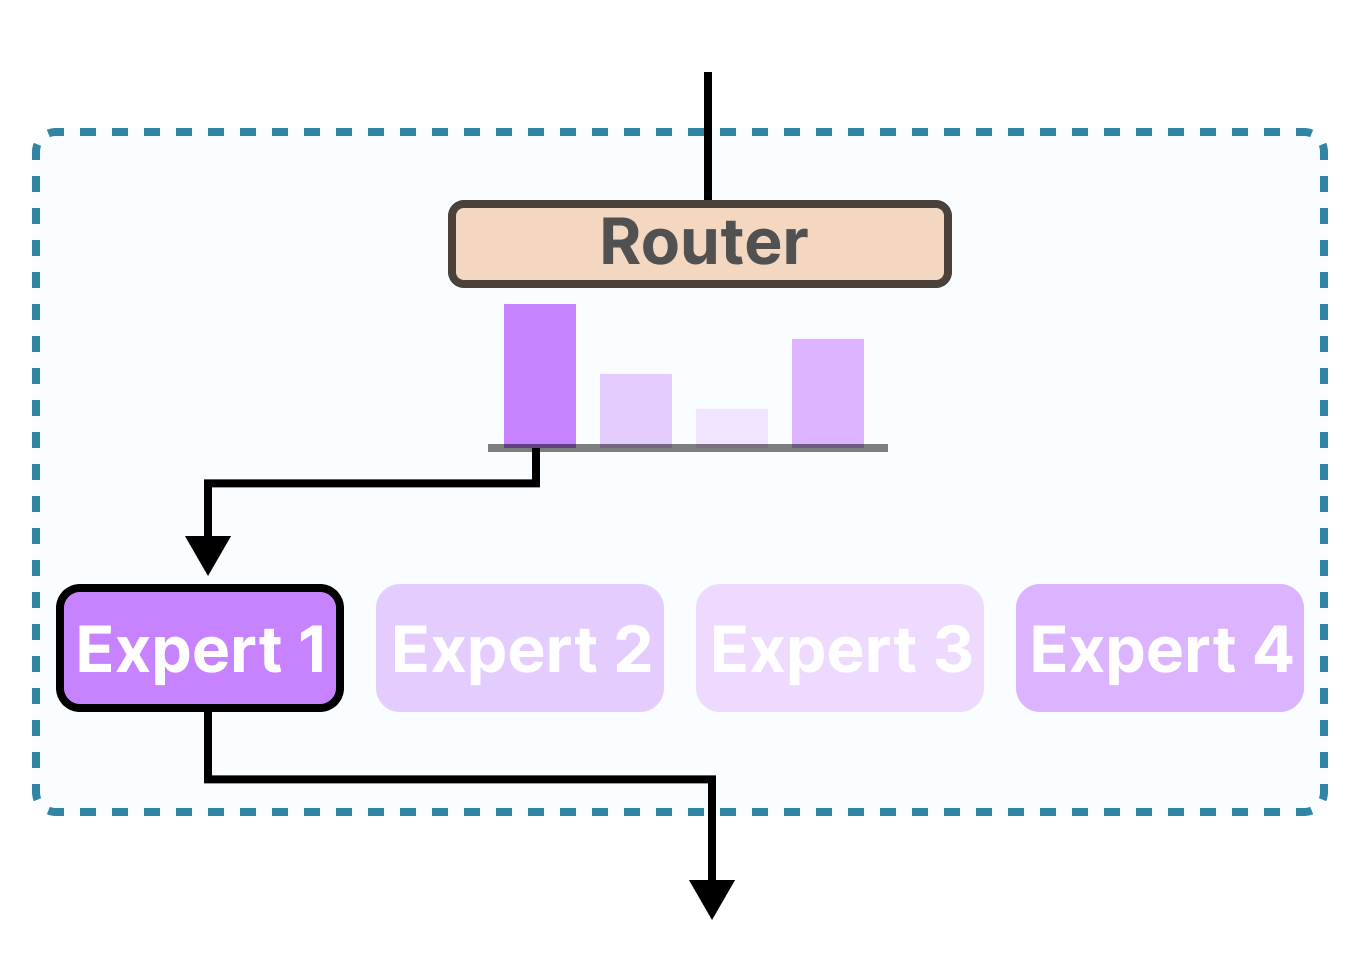
\includegraphics[width=0.7\textwidth]{vmoe.png}
  \caption{Adaptive expert routing in Vision Mixture of Experts.}
  \label{fig:vmoe-routing}
\end{figure}

\section{Conclusion}

This chapter reviewed key advancements in automated skin cancer detection and explored the integration of Mixture of Experts (MoE) models across domains. In the domain of skin cancer detection, several strategies have demonstrated notable improvements in classification performance. Menegola et al. (2017) showed that transfer learning protocols, especially multi-step transfer, significantly improve AUC scores when fine-tuning CNNs for melanoma detection. Ha et al. (2020) introduced an ensemble of EfficientNet models, enhanced with patient metadata and meta-classification, which achieved near state-of-the-art AUCs on both validation and test sets. DiSanto et al. (2022) demonstrated that advanced contextual augmentations yield more robust generalization, particularly on out-of-distribution data.

In the Mixture of Experts domain, Fedus et al. (2021) presented the Switch Transformer for NLP tasks, achieving substantial speedups and scalability through sparse expert activation. Riquelme et al. (2021) extended MoE strategies to vision models with V-MoE, demonstrating adaptive expert routing that improved accuracy while reducing computational cost.

Together, these findings highlight the promise of combining CNN-based backbone  and the potential of MoE architectures for scalable, adaptive learning. In this work, we aim to explore MoE approaches tailored to the dermatology domain, particularly for melanoma classification, with the goal of achieving high diagnostic performance and improved generalization on  dermoscopic datasets.